\documentclass[runningheads]{llncs}

% ---------------------------------------------------------------
% Include basic ECCV package
 
% TODO REVIEW: Insert your submission number below by replacing '*****'
% TODO FINAL: Comment out the following line for the camera-ready version
\usepackage[review,year=2026,ID=4615]{eccv}
% TODO FINAL: Un-comment the following line for the camera-ready version
%\usepackage{eccv}

% OPTIONAL: Un-comment the following line for a version which is easier to read
% on small portrait-orientation screens (e.g., mobile phones, or beside other windows)
%\usepackage[mobile]{eccv}


% ---------------------------------------------------------------
% Other packages

% Commonly used abbreviations (\eg, \ie, \etc, \cf, \etal, etc.)
\usepackage{eccvabbrv}

% Include other packages here, before hyperref.
\usepackage[utf8]{inputenc} % allow utf-8 input
\usepackage[T1]{fontenc}    % use 8-bit T1 fonts
\usepackage{url}            % simple URL typesetting
\usepackage{booktabs}       % professional-quality tables
\usepackage{amsmath}
\usepackage{amsfonts}       % blackboard math symbols
\usepackage{nicefrac}       % compact symbols for 1/2, etc.
\usepackage{microtype}      % microtypography
\usepackage{xcolor}         % colors
\usepackage{comment}
% TODO FINAL: Remove [draft] to render actual images.
\usepackage{graphicx}
\usepackage{multirow}
\usepackage{enumitem}
\usepackage{tabularx}
\usepackage{pifont}
\usepackage[numbers]{natbib}
\usepackage{tikz}
\usetikzlibrary{positioning}

\newcommand{\todo}[1]{\textbf{\color{red}[TODO: #1]}}
\newcommand{\sam}[1]{\textbf{\color{blue}[Sam: #1]}}
\newcommand{\jake}[1]{\textbf{\color{green}[Jake: #1]}}
\newcommand{\gpt}[1]{\textbf{\color{orange}[GPT: #1]}}
\newcommand{\claude}[1]{\textbf{\color{purple}[Claude: #1]}}

\usepackage[detect-all,separate-uncertainty = true]{siunitx}
\sisetup{
    output-exponent-marker=\ensuremath{\mathrm{e}},
    group-separator= {,},
    group-minimum-digits = 4,
    list-final-separator={, },
    mode={math},
    retain-explicit-plus
}

\makeatletter
\renewcommand{\paragraph}{%
  \@startsection{paragraph}{4}%
  {\z@}{1.5ex \@plus 1ex \@minus .2ex}{-0.5em}%
  {\normalfont\normalsize\bfseries}%
}
\makeatother

\setlist{nosep}

%%
%% globally adjusts space between figure and caption
%%
\setlength{\abovecaptionskip}{.5em}


%%
%% Commonly used math definitions
%%
% \DeclareMathOperator*{\argmin}{arg\,min}
% \DeclareMathOperator*{\argmax}{arg\,max}

%% Tigthen underline
\usepackage{soul}
\setuldepth{foobar}

\definecolor{green}{RGB}{25, 169, 116}
\definecolor{red}{RGB}{255, 65, 54}
\newcommand{\cmark}{\textcolor{green}{\ding{51}}}
\newcommand{\xmark}{\textcolor{red}{\ding{55}}}
% For fishvista
\definecolor{blue}{RGB}{0, 18, 115}
\definecolor{cyan}{RGB}{10, 147, 150}
\definecolor{sea}{RGB}{148, 210, 189}

% The "axessiblity" package can be found at: https://ctan.org/pkg/axessibility?lang=en
\usepackage[accsupp]{axessibility}  % Improves PDF readability for those with disabilities.


% ---------------------------------------------------------------
% Hyperref package

% It is strongly recommended to use hyperref, especially for the review version.
% Please disable hyperref *only* if you encounter grave issues.
% hyperref with option pagebackref eases the reviewers' job, but should be disabled for the final version.
%
% If you comment hyperref and then uncomment it, you should delete
% main.aux before re-running LaTeX.
% (Or just hit 'q' on the first LaTeX run, let it finish, and you
%  should be clear).

% TODO FINAL: Comment out the following line for the camera-ready version
\usepackage[pagebackref,breaklinks,colorlinks,citecolor=eccvblue]{hyperref}
% TODO FINAL: Un-comment the following line for the camera-ready version
% \usepackage{hyperref}

% Support for ORCID icon
\usepackage{orcidlink}


\begin{document}

% ---------------------------------------------------------------
% TODO REVIEW: Replace with your title
\title{Towards Open-Ended Visual Scientific Discovery with Sparse Autoencoders} 

% TODO REVIEW: If the paper title is too long for the running head, you can set
% an abbreviated paper title here. If not, comment out.
% \titlerunning{Abbreviated paper title}

% TODO FINAL: Replace with your author list. 
% Include the authors' OCRID for the camera-ready version, if at all possible.
\author{First Author\inst{1}\orcidlink{0000-1111-2222-3333} \and
Second Author\inst{2,3}\orcidlink{1111-2222-3333-4444} \and
Third Author\inst{3}\orcidlink{2222--3333-4444-5555}}

% TODO FINAL: Replace with an abbreviated list of authors.
\authorrunning{F.~Author et al.}
% First names are abbreviated in the running head.
% If there are more than two authors, 'et al.' is used.

% TODO FINAL: Replace with your institution list.
\institute{Princeton University, Princeton NJ 08544, USA \and
Springer Heidelberg, Tiergartenstr.~17, 69121 Heidelberg, Germany
\email{lncs@springer.com}\\
\url{http://www.springer.com/gp/computer-science/lncs} \and
ABC Institute, Rupert-Karls-University Heidelberg, Heidelberg, Germany\\
\email{\{abc,lncs\}@uni-heidelberg.de}}

\maketitle


\begin{abstract}
% Scientific archives now contain hundreds of petabytes of data across genomics, ecology, climate, and molecular biology that could reveal undiscovered patterns if systematically analyzed at scale.
Large-scale weakly-supervised datasets in language and vision have driven the development of foundation models whose internal representations encode rich structure (patterns, co-occurrences and statistical regularities) beyond their training objectives.
Most existing methods extract structure only for pre-specified targets; they excel at confirmation but do not support open-ended discovery of unknown patterns.
% We ask whether sparse autoencoders (SAEs) can enable open-ended concept discovery from foundation model representations.
We evaluate sparse autoencoders (SAEs) as a label-free solution for this problem and evaluate them using controlled rediscovery: we train on unlabeled activations and then test whether the resulting features align with held-out semantic structure.
% We compare against strong label-free alternatives on concept-alignment metrics.
We apply the same procedure to both general domain concept discovery and to ecological imagery, where SAEs surface fine-grained anatomical structure without access to segmentation or part labels, providing a scientific case study with ground-truth validation.
These results validate SAEs as a practical, discovery-oriented instrument for turning opaque vision representations into candidate scientific concepts.
We view this as a prerequisite to, rather than a substitute for, domain-expert validation of truly novel scientific findings.
% While our experiments focus on vision with an ecology case study, the method is domain-agnostic and applicable to models in other sciences (e.g., proteins, genomics, weather).
% Our results indicate that SAEs provide a practical instrument for exploring what scientific foundation models have learned, an important prerequisite for moving beyond purely confirmatory use of foundation models.

% TODO REVIEW: update keywords
\keywords{Sparse Autoencoders \and Concept Discovery \and AI for Science}
\end{abstract}

\section{Introduction}

Scientific data now spans hundreds of petabytes across domains, far outpacing what any lab can annotate or manually inspect.\footnote{For example, the NIH Sequence Read Archive exposes roughly \num{47} PB of public sequencing data, the European Nucleotide Archive provides roughly \num{63} PB of immediately downloadable data, NASA Earthdata (EOSDIS) hosts more than \num{120} PB of open Earth science data, and a single reanalysis, ERA5, is on the order of \num{5} PB.}
Large neural networks trained on these datasets cover proteins (e.g., AlphaFold 3 \citep{abramson2024alphafold3}), weather (e.g., GraphCast, GenCast \citep{lam2023graphcast,price2025gencast}), genomics (e.g., scGPT, ESM3 \citep{cui2024scgpt,hayes2025esm3}), and vision (e.g., Scale-MAE, BioCLIP 2 \citep{reed2023scale,gu2025bioclip2}).
These models achieve strong predictive performance across a variety of tasks by learning compressed representations of the underlying data distribution's structure.
% They learn to organize data by recurring patterns and factors \citep{bommasoni2021opportunities}; in vision, self-supervised encoders demonstrably learn object- and part-level structure that transfers to dense prediction tasks \citep{caron2021dinov1,oquab2024dinov2}.



\begin{figure}[t]
\centering
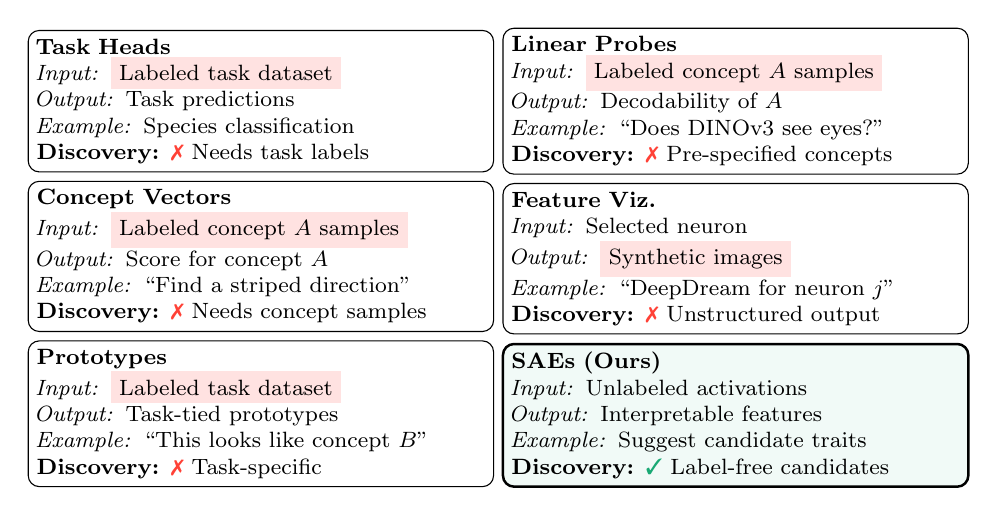
\begin{tikzpicture}[
  font=\footnotesize,
  card/.style={draw, rounded corners, align=left, inner sep=3pt, text width=0.47\columnwidth},
  good/.style={card, line width=0.9pt, fill=green!6},
  gap/.style={}
]

\node[card] (c1) {
  \textbf{Task Heads}\\
  \textit{Input:} \colorbox{red!15}{Labeled task dataset}\\
  \textit{Output:} Task predictions\\
  \textit{Example:} Species classification\\
  \textbf{Discovery:} \textcolor{red}{\xmark} Needs task labels
};

\node[card, right=3pt of c1] (c2) {
  \textbf{Linear Probes}\\
  \textit{Input:} \colorbox{red!15}{Labeled concept $A$ samples}\\
  \textit{Output:} Decodability of $A$\\
  \textit{Example:} ``Does DINOv3 see eyes?''\\
  \textbf{Discovery:} \textcolor{red}{\xmark} Pre-specified concepts
};

\node[card, below=3pt of c1] (c3) {
  \textbf{Concept Vectors}\\
  \textit{Input:} \colorbox{red!15}{Labeled concept $A$ samples}\\
  \textit{Output:} Score for concept $A$\\
  \textit{Example:} ``Find a striped direction''\\
  \textbf{Discovery:} \textcolor{red}{\xmark} Needs concept samples
};

\node[card, below=3pt of c2] (c4) {
  \textbf{Feature Viz.}\\
  \textit{Input:} Selected neuron\\
  \textit{Output:} \colorbox{red!15}{Synthetic images}\\
  \textit{Example:} ``DeepDream for neuron $j$''\\
  \textbf{Discovery:} \textcolor{red}{\xmark} Unstructured output
};

\node[card, below=3pt of c3] (c5) {
  \textbf{Prototypes}\\
  \textit{Input:} \colorbox{red!15}{Labeled task dataset}\\
  \textit{Output:} Task-tied prototypes\\
  \textit{Example:} ``This looks like concept $B$''\\
  \textbf{Discovery:} \textcolor{red}{\xmark} Task-specific
};

\node[good, below=3pt of c4] (c6) {
  \textbf{SAEs (Ours)}\\
  \textit{Input:} Unlabeled activations\\
  \textit{Output:} Interpretable features\\
  \textit{Example:} Suggest candidate traits\\
  \textbf{Discovery:} \textcolor{green!50!black}{\cmark} Label-free candidates
};

\end{tikzpicture}
\caption{Comparison of methods for extracting knowledge from foundation models. 
    Most approaches require researchers to specify concepts or tasks in advance, limiting them to confirmatory analysis. 
    SAEs support open-ended feature discovery by surfacing the model's learned feature vocabulary in a structured format without any supervision.}\label{fig:related-work}
\end{figure}

However, current usage of such foundation models in science is predominantly task-centric: models are used as frozen feature extractors or fine-tuned for specific predictions (species classification \citep{vanhorn2021inat21}, cellular responses to perturbations \citep{roohani2025vcc}, 3-D protein structure \citep{haas2018continuous,pereira2021high}).
The learned, compressed representations are high-dimensional embeddings optimized for task performance.
While these representations enable accurate predictions, they do not directly provide reusable scientific measurements or expose the structure the model learned for systematic investigation.
This limits foundation models to \emph{confirmatory} applications where the target concepts are pre-specified (see \cref{fig:related-work}).

\paragraph{Discovery vs. Confirmation}
Scientific discovery often involves establishing names and descriptions of previously unexplained phenomena in the world \citep{kuhn1970structure}.
A morphological feature that distinguishes subspecies but is not formally cataloged, an unexplored correlation between climate variables, or a sequence motif in an understudied protein family: these cannot be found by methods that require specifying target concepts in advance.

Foundation models trained on millions of samples have seen and learned from more data than any human could.
If such models have learned semantic patterns not captured by existing annotations, interpretability methods offer a route to systematically surface this learned structure.
% The patterns are encoded in the model's representations: model interpretability offers a path towards unlocking model-learned discoveries.
However, current interpretability approaches require specifying concepts:
\begin{itemize}
\item{Supervised probing tests for known concepts \citep{alain2016understanding}.}
\item{Concept activation vectors (CAV) test for user-defined concepts \citep{kim2018tcav}.}
\item{Saliency and attention explain single task-specific predictions \citep{selvaraju2017gradcam,sundararajan2017axiomatic,simonyan2013deep}.}
\end{itemize}
These methods excel at \textit{confirmation}, but cannot explore representation space to generate hypotheses about model-learned patterns.
When labels are scarce and salient factors are unknown (i.e., in scientific use cases), the inability to extract unnamed patterns from foundation models represents a significant limitation.
If foundation models have learned meaningful patterns from data that exceed what humans can manually analyze, we need methods to surface those patterns without pre-specification \citep{hughes2024open}.
We view the method of surfacing candidate features for human validation as a prerequisite step toward scientific discovery.

% Yet discovery-oriented methods face a basic evaluation problem: if the interesting factors are genuinely unknown, there is no ground-truth label against which to score them. 
% We therefore separate deployment from validation. 
% Therefore, we aim to validate methods through controlled rediscovery: training on unlabeled activations and testing whether the surfaced features align with known but withheld structure. 
% Success in this setting is not sufficient for new scientific discovery, but it is a necessary and testable prerequisite.



\begin{figure*}[t]
    \centering
    \includegraphics[width=\linewidth]{figures/hook.png}
    % \includegraphics[width=\linewidth]{figures/hook.pdf}
    \caption{\textit{Validating an instrument for open-ended feature discovery.} 
    \textbf{Left:} Typical use of a foundation model in science: an input image is passed through a pretrained encoder and a task-specific head to yield class scores; the dense representation remains an opaque embedding, so unnamed factors are inaccessible. 
    \textbf{Right:} Our procedure composes a foundation model with a sparse autoencoder, producing a library of interpretable semantic concepts with per-example activation maps. 
    We find that these concepts align with and localize anatomical parts (e.g., head, dorsal fin) without seeing part-of-body labels.
    Fish images are shown as a case study with known anatomy providing a controlled rediscovery test; the explored method is domain-agnostic.
    }\label{fig:hook}
    \vspace{-6pt}
\end{figure*}

\paragraph{Our approach.}
To address this gap, we study sparse autoencoders (SAEs) as a candidate mechanism for decomposing foundation model representations into interpretable features without concept supervision \citep{bricken2023monosemanticity,templeton2024scaling,cunningham2023sparse,gao2025scaling}.
SAEs learn an overcomplete dictionary that reconstructs model activations through sparse linear combinations, with sparsity encouraging individual features to capture coherent semantic units.
Unlike supervised methods, SAEs require no concept labels during training.
Each learned feature provides a per-example activation score together with its decoding direction and exemplar evidence, enabling systematic investigation of what patterns the model represents.
In short, we treat SAEs as a candidate tool for open-ended feature discovery from foundation models and seek to rigorously evaluate that tool in controlled settings \citep{peng2025unknown}.
A discovery-oriented method cannot be evaluated directly on unknown unknowns; before deploying such a method in truly open-ended settings, we must first test whether it can reliably recover known but withheld structure without concept supervision.

\paragraph{Evidence.}
We train SAEs on patch-level activations from DINOv3 \citep{simeoni2025dinov3} and Perception Encoder \citep{bolya2025perception}, two large pre-trained vision transformer \citep[ViT;][]{dosovitskiy2020vit} backbones.
We evaluate if SAEs can recover fine-grained semantic structure without access to labels in two settings: (1) ADE20K scene segmentation \citep{zhou2017ade20k}, containing \num{150} object classes, and (2) ecological images, where we test recovery of anatomical body parts from the FishVista dataset \citep{mehrab2024fishvista,fishvistadataset}.
Both settings provide labeled semantic structure, so they serve as controlled rediscovery tests of recovering concepts that domain experts already recognize.
We find that SAEs extract semantic concepts that were never explicitly labeled in DINOv3's self-supervised training objective, as assessed by alignment to held-out labels in the evaluation sets.
We compare against standard label-free decomposition baselines ($k$-means clustering, PCA and semi-nonnegative matrix factorization \citep[SemiNMF;][]{ding2008convex}) and find that SAEs achieve substantially higher concept alignment: even a standard ReLU SAE covers \num{26.4}\% of ADE20K classes at our AP threshold, compared to \num{7.9}\% for the best baseline (see \cref{sec:ade20k,sec:ablations} for details).

Our results indicate that unsupervised sparse decomposition can recover semantic structure from foundation model representations in controlled rediscovery settings.
On standard vision benchmarks, SAEs rediscover segmentation classes and spatial relationships without label access during training.
On scientific images, they surface fine-grained anatomical features, providing measurable quantities that can be evaluated against biological annotations.
We analyze when this approach succeeds and when it fails, documenting sensitivity to architectural choices, layer selection, and dataset characteristics.

The contribution of this work is conceptual and evaluative rather than methodological or biological: we propose and validate a new role for interpretability in science. 
Rather than explaining a model's prediction (a standard interpretability goal), we show that SAEs can generate hypotheses, converting opaque foundation-model representations into candidate concepts that domain experts can inspect and validate. 
Our controlled rediscovery experiments provide feasibility-level evidence that SAEs surface semantic structure that was never labeled during training, outperforming standard unsupervised alternatives. 
We focus on validating the instrument in controlled settings where ground truth exists; applying it to generate novel scientific hypotheses requires domain-specific follow-up (e.g., in proteins \citep{abramson2024alphafold3}, genomics \citep{cui2024scgpt} and weather \citep{lam2023graphcast}), which we leave to future work.
We view our work as a necessary prerequisite step: establish that SAEs can recover known structure before using them to search for novel scientific phenomena.

\section{Related Work}


\paragraph{Foundation Models.}
Domain-specific foundation models capture rich structure and achieve state-of-the-art performance on their focal tasks, as shown in proteins \citep{abramson2024alphafold3,hayes2025esm3}, ecology \citep{stevens2024bioclip}, weather \citep{lam2023graphcast,price2025gencast}, and single-cell genomics \citep{cui2024scgpt}.
In both general and scientific domains, large-scale training leads to emergent abilities beyond the pre-training objective \citep{wei2022emergent,gu2025bioclip2}.
Theory and evidence suggest that large pretrained models internalize meaningful structure \citep{ha2018world,caron2021dinov1,lecun2022jepa,huh2024platonic}.
Despite this, most scientific models are benchmarked as \textbf{task-specific predictors} rather than sources of novel concepts.

\paragraph{Interpretability Methods.}
A large body of work explains predictions without exposing a global factorization of representations.
Saliency and attribution methods (e.g., gradients, Integrated Gradients, Grad-CAM) highlight input regions for \emph{individual} decisions and have known validity pitfalls \citep{simonyan2013deep,sundararajan2017axiomatic,selvaraju2017gradcam,adebayo2018sanity}.
Linear probes test separability of \emph{pre-specified} targets \citep{alain2016understanding,hewitt2019probes}; concept methods such as TCAV/ACE require exemplar sets and so test investigator-defined ideas \citep{kim2018tcav,ghorbani2019ace}.
Prototype models (ProtoPNet, ProtoTree, ProtoPFormer) provide case-based, class-tied explanations but are trained end-to-end for specific tasks \citep{chen2019protopnet,nauta2021prototree,xue2022protopformer}.
Activation maximization and “feature visualization” (DeepDream-style) optimize inputs for chosen units to aid intuition, but produce synthetic, non-natural images \citep{mahendran2016visualizing,nguyen2016dgn,olah2017feature}.
These approaches excel at explaining predictions or testing for known concepts (confirmation) but cannot be used to discover patterns without prior specification.

\paragraph{Sparse Autoencoders \& Decomposition.}
Classical dictionary learning and sparse coding demonstrated that sparse, parts-based factors can emerge from natural data \citep{olshausen1996nature,aharon2006ksvd,lee1999nmf}.
Recent work applies sparse autoencoders (SAEs) to model activations, showing that sparse decompositions can partially ``unmix'' superposed features and yield monosemantic directions \citep{elhage2022superposition,bricken2023monosemanticity,gao2025scaling} in language and vision models.
SAEs address the superposition hypothesis \citep{elhage2022superposition} by assigning features to directions in activation space rather than individual neurons.
\citep{gao2025scaling} demonstrate that $k$-sparse autoencoders scale effectively and improve reconstruction--sparsity tradeoffs.
Concurrent work argues for using SAEs for discovering unknown concepts rather than acting on known ones \citep{peng2025unknown} and applies dictionary learning to microscopy foundation models for biological concept extraction \citep{donhauser2024towards}.
Beyond SAEs, concept factorization methods such as CRAFT and related work use NMF-like decompositions to extract human-interpretable concepts and quantify their importance \citep{fel2023craft,fel2023holistic}.
% Hierarchical SAE variants have also been applied to vision-language models for structured concept extraction \citep{zaigrajew2025interpretingclip}.
Finally, recent analyses highlight stability and identifiability limits of SAE dictionaries across runs \citep{leask2025sparse}, motivating careful evaluation protocols.
% However, systematic evaluation of SAEs for semantic concept recovery on standard benchmarks, comparison to classical decomposition baselines, and application to scientific discovery with ground-truth validation remains limited.

\paragraph{Discovery.}
We use \emph{discovery} to mean surfacing previously unnamed factors (morphological features distinguishing subspecies, correlations between climate variables, or conserved sequence motifs in understudied proteins) as opposed to \emph{confirmation} of pre-specified targets.
Closest in intent to our goal are (i) work advocating SAEs for uncovering \emph{unknown} concepts rather than acting on \emph{known} ones \citep{peng2025unknown}, (ii) dictionary-learning approaches that extract biological concepts from microscopy foundation models \citep{donhauser2024towards}, and (iii) automated concept discovery pipelines that discover concepts and then name or validate them with limited supervision \citep{rao2024discover}.
We differ by targeting dense token representations in vision and validating both on a standard semantic benchmark and a scientific ecology case study.
We also differ from unsupervised dense segmentation methods (LOST, TokenCut, STEGO, MaskCut) by returning global features with per-patch activations rather than per-image masks or clusters \citep{simeoni2021lost,wang2023tokencut,hamilton2022stego,wang2023maskcut}.

Methods for open-ended, unsupervised discovery from foundation model representations remain underdeveloped.
Our work takes a step toward addressing this gap by demonstrating, in controlled rediscovery settings, that sparse decomposition of foundation model representations can systematically surface semantic structure.

\section{Methodology}

We ask the question: ``Can SAEs reliably rediscover unlabeled concepts in pre-trained models?''
Because discovery demands finding unnamed structure rather than confirming known categories, our method avoids concept supervision and treats labels only as holdout probes.
Our goal is to recover a dictionary whose latents serve as candidate concepts and other interpretable features that can be measured and compared across images.
We outline the ViT feature extraction, the SAE objective, and the evaluation probes that operationalize this goal.

\paragraph{Foundation Model.} We use the publicly available DINOv3 ViT-L/16 checkpoint \citep{simeoni2025dinov3}.
Images are resized with an aspect-ratio-aware transform that enforces exactly \num{256} patches per image (a $h\times w$ patch grid with $hw=256$ chosen to minimize aspect-ratio distortion), instead of forcing square $256\times256$ inputs.
We extract patch-token activations ([CLS] discarded) from the final (24th) layer. 
% We expect the later half of ViT layers to contain the best features \citep{bolya2025perceptionencoder}; in all experiments, we sweep over \num{6} evenly-spaced layers: for \num{24}-layer ViT-L models, we use layers \num{14}, \num{16}, \num{18}, \num{20}, \num{22}, and \num{24}.\footnote{For \num{12}-layer ViT-S and ViT-B models, we use the last \num{6} layers: \num{7}, \num{8}, \num{9}, \num{10}, \num{11}, and \num{12}.}

\paragraph{Sparse Autoencoders (SAEs).} 
Our dictionary learner is a ReLU SAE \citep{bricken2023monosemanticity,templeton2024scaling}; given a $d$-dimensional activation vector $\mathbf{x} \in \mathbb{R}^d$ from an intermediate layer $l$ of a transformer, an SAE maps $\mathbf{x}$ to a sparse representation $f(\mathbf{x})$ (\cref{eq:enc,eq:act}) and reconstructs the original input (\cref{eq:dec}):
\begin{align}
    \mathbf{h} &= W_\text{enc} (\mathbf{x} - b_\text{dec}) + b_\text{enc} \label{eq:enc} \\
    f(\mathbf{x}) &= \text{ReLU}(\mathbf{h}) \label{eq:act} \\
    \mathbf{\hat{x}} &= W_\text{dec} f(\mathbf{x}) + b_\text{dec} \label{eq:dec}
\end{align}
where $W_\text{enc} \in \mathbb{R}^{n \times d}$, $b_\text{enc} \in \mathbb{R}^{n}$, $W_\text{dec} \in \mathbb{R}^{d \times n}$ and $b_\text{dec} \in \mathbb{R}^{d}$.
The training objective minimizes reconstruction error while encouraging sparsity:
\begin{equation}
    \mathcal{L}(\theta) = ||\mathbf{x} - \mathbf{\hat{x}}||_2^2 + \lambda \mathcal{S}(f(\mathbf{x}))
\end{equation}
where $\lambda$ controls the sparsity penalty and $\mathcal{S}$ measures sparsity (L$_1$ norm for training, L$_0$ for model selection).

We train \num{16384}-latent SAEs for 100M patches and sweep a logarithmic grid of sparsity coefficients $\lambda$ and learning rates.
We summarize each trained model by its reconstruction quality (normalized MSE) and sparsity (L$_0$).
% normalized_mse (float): reconstruction sum squared SAE error / reconstruction sum squared mean baseline error
Normalized MSE (NMSE) is MSE normalized by a mean baseline MSE:
\begin{equation}\label{eq:nmse}
\text{NMSE} = \frac{\sum_i || \mathbf{x_i} - \mathbf{\hat{x}_i} ||_2^2}{\sum_i || \mathbf{x_i} - \mathbf{\bar{x}} ||_2^2}
\end{equation}
where $\mathbf{\hat{x}_i}$ is the predicted reconstruction and $\mathbf{\bar{x}}$ is the mean of all $\mathbf{x_i}$.



\begin{figure}[t]
    \centering
    \small
    \small
    \centering
    \begin{subfigure}[b]{0.48\textwidth}
        \includegraphics[width=\linewidth]{figures/dinov3_vitl16_in1k_baselines.pdf}
    \end{subfigure}
    \hfill
    \begin{subfigure}[b]{0.48\textwidth}
        \centering
        \includegraphics[width=\linewidth]{figures/dinov3_vitl_layers_in1k_sae.pdf}
    \end{subfigure}
    \caption{\textbf{(Left)} We compare $k$-means, PCA, SemiNMF and SAEs along the reconstruction--sparsity tradeoff for learning to decompose ViT patch activations. We use final layer activations from DINOv3 ViT-L/16 on ImageNet-1K; we fit all methods on the training split and measure normalized MSE (see \cref{eq:nmse}) and L$_0$ on the validation split. For $k$-means, we ``reconstruct'' every patch with its nearest centroid; thus, L$_0$ is always $1$. For PCA, we sweep the number of components. We sweep $\lambda$ for the SAE and show the Pareto frontier of reconstruction--sparsity. \textbf{Takeaway:} Reconstruction--sparsity does not indicate an optimal method.
    \textbf{(Right)} Layer-wise reconstruction–sparsity trade-off (DINOv3 ViT-L/16) on ImageNet-1K. Each curve is a ViT layer. Later layers consistently incur higher MSE at matched sparsity, indicating greater representational complexity. Note that the $y$-axis is \textit{raw} rather than normalized MSE.
    }\label{fig:baseline-pareto+layerwise}
\end{figure}

\begin{figure*}[t]
    \small
    \centering
    \begin{subfigure}[b]{0.23\textwidth}
        \centering
        \includegraphics[width=0.48\textwidth]{figures/kmeans-ade20k-person-1.png}
        \hfill
        \includegraphics[width=0.48\textwidth]{figures/kmeans-ade20k-toilet-1.png}
        \includegraphics[width=0.48\textwidth]{figures/kmeans-ade20k-person-2.png}
        \hfill
        \includegraphics[width=0.48\textwidth]{figures/kmeans-ade20k-toilet-2.png}
        \includegraphics[width=0.48\textwidth]{figures/kmeans-ade20k-person-3.png}
        \hfill
        \includegraphics[width=0.48\textwidth]{figures/kmeans-ade20k-toilet-3.png}
        \includegraphics[width=0.48\textwidth]{figures/kmeans-ade20k-person-4.png}
        \hfill
        \includegraphics[width=0.48\textwidth]{figures/kmeans-ade20k-toilet-4.png}
        \caption{$k$-means}
        \label{fig:ade20k-examples-kmeans}
    \end{subfigure}
    \hfill
    \begin{subfigure}[b]{0.23\textwidth}
        \centering
        \includegraphics[width=0.48\textwidth]{figures/pca-ade20k-person-1.png}
        \hfill
        \includegraphics[width=0.48\textwidth]{figures/pca-ade20k-toilet-1.png}
        \includegraphics[width=0.48\textwidth]{figures/pca-ade20k-person-2.png}
        \hfill
        \includegraphics[width=0.48\textwidth]{figures/pca-ade20k-toilet-2.png}
        \includegraphics[width=0.48\textwidth]{figures/pca-ade20k-person-3.png}
        \hfill
        \includegraphics[width=0.48\textwidth]{figures/pca-ade20k-toilet-3.png}
        \includegraphics[width=0.48\textwidth]{figures/pca-ade20k-person-4.png}
        \hfill
        \includegraphics[width=0.48\textwidth]{figures/pca-ade20k-toilet-4.png}
        \caption{PCA}
        \label{fig:ade20k-examples-pca}
    \end{subfigure}
    \hfill
    \begin{subfigure}[b]{0.23\textwidth}
        \centering
        \includegraphics[width=0.48\textwidth]{figures/seminmf-ade20k-person-1.png}
        \hfill
        \includegraphics[width=0.48\textwidth]{figures/seminmf-ade20k-toilet-1.png}
        \includegraphics[width=0.48\textwidth]{figures/seminmf-ade20k-person-2.png}
        \hfill
        \includegraphics[width=0.48\textwidth]{figures/seminmf-ade20k-toilet-2.png}
        \includegraphics[width=0.48\textwidth]{figures/seminmf-ade20k-person-3.png}
        \hfill
        \includegraphics[width=0.48\textwidth]{figures/seminmf-ade20k-toilet-3.png}
        \includegraphics[width=0.48\textwidth]{figures/seminmf-ade20k-person-4.png}
        \hfill
        \includegraphics[width=0.48\textwidth]{figures/seminmf-ade20k-toilet-4.png}
        \caption{SemiNMF}
        \label{fig:ade20k-examples-seminmf}
    \end{subfigure}
    \hfill
    \begin{subfigure}[b]{0.23\textwidth}
        \centering
        \includegraphics[width=0.48\textwidth]{figures/vanilla-ade20k-person-1.png}
        \hfill
        \includegraphics[width=0.48\textwidth]{figures/vanilla-ade20k-toilet-1.png}
        \includegraphics[width=0.48\textwidth]{figures/vanilla-ade20k-person-2.png}
        \hfill
        \includegraphics[width=0.48\textwidth]{figures/vanilla-ade20k-toilet-2.png}
        \includegraphics[width=0.48\textwidth]{figures/vanilla-ade20k-person-3.png}
        \hfill
        \includegraphics[width=0.48\textwidth]{figures/vanilla-ade20k-toilet-3.png}
        \includegraphics[width=0.48\textwidth]{figures/vanilla-ade20k-person-4.png}
        \hfill
        \includegraphics[width=0.48\textwidth]{figures/vanilla-ade20k-toilet-4.png}
        \caption{SAE}
        \label{fig:ade20k-examples-sae}
    \end{subfigure}
    \caption{   
    Top images for lowest-loss probes for ``person'' (left) and ``toilet'' (right) classes for each method.
    \textbf{(a):} $k$-means does not recover the ``person'' class; the best ``person'' cluster fires on roads.
    \textbf{(b):} PCA learns a ``person'' component, but does not consistently activate on the entire person. Furthermore, PCA does not recover the ``toilet'' class; the best ``toilet''  doesn't have an obvious semantic concept. 
    \textbf{(c):} Semi-nonnegative matrix factorization (SemiNMF) is a strong baseline and learns both ``person'' and ``toilet'' concepts.
    \textbf{(d):} SAEs reliably recover both ``person'' and ``toilet'' and activate on the entire object.
    \textbf{Takeaway}: While $k$-means and PCA are good by dictionary learning metrics, visual concepts recovered by SAEs are more consistent and salient.
    }\label{fig:ade20k-examples}
\end{figure*}



\section{Experiments}\label{sec:experiments}

Our goal is to validate SAEs as an instrument for surfacing semantic structure from foundation models without concept supervision.
The central challenge is evaluating an open-ended discovery method: if the interesting patterns are unknown, how do we measure whether the method finds them?
We address this via \textbf{controlled rediscovery}, training SAEs on unlabeled activations and then testing whether the learned features align with ground-truth concepts that were withheld during training.
Strong alignment on known concepts gives confidence that the same procedure will surface meaningful structure where ground truth is unavailable.

We first establish that SAEs outperform label-free baselines ($k$-means, PCA, and SemiNMF) at recovering segmentation concepts on ADE20K, a standard benchmark with 150 classes (\cref{sec:ade20k}).
We then ablate design choices to understand what drives rediscovery (\cref{sec:ablations}).
Finally, we apply the best configuration to an ecological case study on fish anatomy, testing whether the same procedure surfaces fine-grained biological structure (\cref{sec:fishvista}).
% We also report the reconstruction--sparsity trade-off (normalized MSE vs.\ L$_0$) throughout.

For discovery, a researcher must be able to inspect individual features and judge what each one represents.
This requires monosemantic features: each latent should track a single coherent concept.
We implement this with 1-D logistic probes, the standard evaluation in the SAE literature \citep{gao2025scaling}: for each concept, we fit a binary logistic on each latent $i$'s activation $z_i$ and select the best latent per class:
\begin{equation}\label{eq:probe-loss}
    \min_{i,w,b} \mathbb{E} \big[-y \log \sigma (wz_i + b) - (1-y) \log (1 - \sigma (wz_i+b)) \big]
\end{equation}
Because the probe is axis-aligned by design, it favors representations whose individual axes carry semantic meaning.
This is not a limitation of the evaluation but a requirement of the use case: features that cannot be understood one at a time cannot be browsed for discovery.
We report (1) probe $R$: loss $\mathcal{L}$ normalized by a bias-only baseline $\mathcal{L}_\pi$: $1 - (\mathcal{L}/\mathcal{L}_\pi)$, (2) mean Average Precision (mAP) across all classes, (3) Purity@$k$: precision of the top-$k$ activated patches for each feature, and (4) Coverage@$\tau$: the fraction of classes whose best-aligned feature achieves AP $\geq \tau$.
We select the SAE with the best probe loss on the training split and report validation metrics.



\begin{table}[t]
    \centering
    \small
    % \setlength{\tabcolsep}{3pt}
    \caption{SAEs vs.\ unsupervised baselines for rediscovering ADE20K's semantic segmentation classes from DINOv3 ViT-L/16.
    For each method, we choose the best layer from DINOv3 based on probe loss (\cref{eq:probe-loss}) on ADE20K's training split and report ADE20K validation metrics.
    Probe $R$ is normalized probe loss, as described in \cref{sec:experiments}.
    Purity@$k$ is precision over the top-$k$ highest-scoring patches for a feature, where $k=16$.
    Coverage@$\tau$ is the fraction of ADE20K classes with best AP $\geq\tau$, where $\tau= 0.3$.
    \textbf{Takeaway:} Even a vanilla ReLU SAE improves downstream concept rediscovery over traditional unsupervised methods, despite comparable reconstruction metrics.
    }\label{tab:ade20k}
    \setlength{\tabcolsep}{3pt}
    \begin{tabular}{l rr rr rrrr}
    \toprule
    & \multicolumn{2}{c}{Source Recon.\ $\downarrow$} & \multicolumn{2}{c}{Target Recon.\ $\downarrow$} & \multicolumn{4}{c}{Downstream $\uparrow$} \\
    \cmidrule(lr){2-3} \cmidrule(lr){4-5} \cmidrule(lr){6-9}
    Method & NMSE & L$_0$ & NMSE & L$_0$ & Probe $R$ & mAP & Pur@$k$ & Cov@$\tau$ \\
    \midrule
    $k$-Means & 0.508 & \textbf{1} & 0.618 & \textbf{1} & 0.001 & 0.031 & \textbf{0.795} & 0.026 \\  % myy5btgw, layer 24/24
    PCA & 0.288 & 256 & 0.352 & 256 & 0.259 & 0.093 & 0.612 & 0.079 \\ % a1x1laxm, 24/24
    SemiNMF & 0.298 & 256 & 0.363 & 256 & 0.209 & 0.088 & 0.696 & 0.079 \\
    % NMF \\
    \midrule
    SAE & \textbf{0.166} & 379.2 & \textbf{0.211} & 379.2 & \textbf{0.441} & \textbf{0.224} & 0.748 & \textbf{0.264} \\  % 0pdum8cq, layer 24/24
    \bottomrule
    \end{tabular}
\end{table}



\subsection{Rediscovering Semantic Segmentations}\label{sec:ade20k}

We use ADE20K (150 classes) as a standard testbed for controlled rediscovery: can label-free SAE features align with segmentation classes? 
SAEs are trained on ImageNet-1K activations only; ADE20K labels enter solely at evaluation, isolating extraction from supervision.
Concretely, we extract activations on ImageNet-1K (train/val) and ADE20K (train/val) from the final layer of DINOv3 ViT-L/16. 


\paragraph{Baseline Methods.}
We compare SAEs to standard unsupervised baselines: $k$-means, principal component analysis (PCA), and semi-nonnegative matrix factorization \citep[SemiNMF;][]{ding2008convex}.
We fit all baselines on ImageNet-1K training activations.
For $k$-means, we use $k$=\num{16384} clusters and use the nearest cluster as the predicted reconstruction with a fixed L$_0$=$1$.
We fit PCA with $n$ components $n \in \{1,4,16,64,256,1024\}$.
For SemiNMF, we use a mini-batch semi-NMF estimator with nonnegative codes and an unconstrained dictionary; codes are inferred by multiplicative updates with cached positive/negative Gram terms, while the dictionary is updated from accumulated $Z^\top Z$ and $Z^\top A$ statistics with a ridge term.
For all methods, we report normalized reconstruction MSE on ImageNet-1K (validation split).
See \cref{app:baselines} for more details.

\paragraph{Results.}
We compare all methods on the reconstruction--sparsity tradeoff in \cref{fig:baseline-pareto+layerwise}, report rediscovery metrics in \cref{tab:ade20k} and show qualitative examples in \cref{fig:ade20k-examples}.
SAEs do not improve upon classical baselines by normalized MSE and sparsity, but \textit{do} lead to better concept discovery as measured by mAP, Purity@$k$ and Coverage@$\tau$.

\paragraph{Discussion.}
$k$-means and PCA are competitive on reconstruction--sparsity trade-offs, yet underperform SAEs on downstream concept-alignment metrics such as mAP, Purity@$k$, and Coverage@$\tau$. 
This reinforces that normalized MSE and L$_0$ measure how well activations are compressed, not how well individual latents track semantic concepts.
Prior work in evaluating SAEs for language model interpretability also finds dictionary-learning metrics insufficient \citep{karvonen2025saebench}.
% For discovery-oriented use, we therefore select SAEs by downstream metrics rather than by reconstruction.

% For size, I am doing ViT-S, ViT-B and ViT-L on IN1K/ADE20K.
% For width, I'm happy to do 1024 x {2, 4, 8, 16, 32} with ViT-L on IN1K/ADE20K.
% For resolution I'm using a ViT-S for storage reasons and am doing 256 patches/img (default), then 576, then 1024. All of them use a native resize that picks out a size that minimizes aspect ratio distortion. So the 256 patch images can be 16 x 16 patches, 8 x 32 patches, 32 x 8 patches, etc. The 576 can be 24 x 24 patches, 32 x 18 patches, 18 x 32 patches, 48 x 12 etc. Then the 1024 can be 32 x 32 patches, etc. 
% 
% Remember, each of these ablations need to measure two things: dictionary learning quality (for completeness) and downstream metrics, BECAUSE WE WANT TO ENABLE DISCOVERY. I think it's very important to emphasize the effects of these ablations on discovery-related metrics rather than NMSE/L$_0$.



\subsection{Ablation Study}\label{sec:ablations}

We ablate ViT size, ViT layer, ViT family and SAE variants to understand what drives concept rediscovery on ADE20K.

\paragraph{Model size.}\label{sec:ablation-size}
Model scale consistently correlates with downstream performance \citep{kaplan2020scaling,hoffmann2022training}.
Prior work proposes scaling laws for SAE reconstruction based on both SAE and foundation model size \citep{gao2025scaling} but does not investigate downstream performance.
We assess foundation model size effects by training SAEs on patch activations from DINOv3 ViT-S/16, ViT-B/16, and ViT-L/16 checkpoints.
The models vary in both total parameter count (\num{22}M, \num{86}M and \num{303}M, respectively) and the embedding dimension $d$ (\num{384}, \num{768}, and \num{1024}, respectively).
% \sam{Because of the difference in embedding dimension, I think smaller $d$ should lead to sparse SAEs, because there's a lower-dimension orthogonal basis or something. @Jake it would be great to get your math background here.} 
% \jake{$d$ actually might not have an impact on the sparsity of your latent. The only thing that enforces the sparsity of your latent is your coefficient, and so its probably more dictated by the complexity of your feature manifold rather than the dimension it's in. This is something that would likely need it's own investigation/paper, so it may be best to avoid making claims about how each difference between models actually impacts discovery. Instead, we could just stick to "bigger = better"}
For each size, we keep the SAE width fixed at \num{16384}, train on ImageNet-1K \num{100}M patch activations and probe the SAEs for ADE20K features.


In \cref{fig:ablations-size+layers} we see that larger models are in fact harder to reconstruct (note that the $y$-axis is \textit{raw} rather than normalized MSE), consistent with prior work in scaling SAEs for language models \citep{gao2025scaling}.
Despite more challenging dictionary learning, we see in \cref{tab:vit-size} that SAEs applied to larger models both recover more concepts (coverage) and are more precise (purity).
All three sizes of the DINOv3 ViTs are distilled from a single, larger teacher model \citep{simeoni2025dinov3}; we conjecture then that all three checkpoints have learned the same set of concepts.
% \sam{I don't know what to make of this. Why is it easier to recover from larger ViTs?} 
These results indicate that, at least for vision, strong foundation models in combination with SAEs can rediscover semantic concepts, which we view as a prerequisite for scientific discovery.
% \todo{Motivated by this, we train SAEs on DINOv3 ViT-7B/16.}


\begin{table}[t]
    \centering
    \small
    \setlength{\tabcolsep}{3pt}
    \caption{
        SAEs on different sizes of DINOv3 for rediscovering ADE20K's semantic segmentation classes.
        Source Recon.\ measures reconstruction on the SAE's training distribution (IN1K); Target Recon.\ measures transfer to the evaluation domain (ADE20K).
        \textbf{Takeaway:} While larger ViTs are harder to reconstruct, they lead to better concept rediscovery.
    }
    \label{tab:vit-size}
    \begin{tabular}{l rr rr rrrr}
    \toprule
    \multirow{2.4}*{ViT} & \multicolumn{2}{c}{Source Recon.\ $\downarrow$} & \multicolumn{2}{c}{Target Recon.\ $\downarrow$} & \multicolumn{4}{c}{Downstream $\uparrow$} \\
    \cmidrule(lr){2-3} \cmidrule(lr){4-5} \cmidrule(lr){6-9}
     & NMSE & L$_0$ & NMSE & L$_0$ & Probe $R$ & mAP & Pur@$k$ & Cov@$\tau$ \\
    \midrule
    ViT-S/16 & \textbf{0.194} & 130.8 & \textbf{0.214} & 130.8 & 0.391 & 0.237 & 0.773 & 0.344 \\  % 5ewxrjg4, layer 12/12
    ViT-B/16 & 0.257 & \textbf{123.8} & 0.283 & \textbf{123.8} & \textbf{0.422} & 0.331 & 0.783 & 0.483 \\  % 6crsj9gj, layer 12/12
    ViT-L/16 & 0.215 & 159.2 & 0.267 & 159.2 & 0.391 & \textbf{0.392} & \textbf{0.798} & \textbf{0.615} \\  % extl56w1, layer 24/24
    \bottomrule
    \end{tabular}
\end{table}


A potential confounder is total training FLOPs: prior work shows that additional SAE training compute (total FLOPs) leads to stronger SAEs as measured by the reconstruction--sparsity tradeoff \citep{gao2025scaling}.
Our SAEs trained on larger embedding dimensions $d$ use more compute during training; this could explain the stronger results for larger models.
However, our SAEs trained on larger models have \textit{worse} reconstruction--sparsity but \textit{better} downstream concept alignment metrics.
% These findings suggest a fundamental tension between reconstruction quality and semantic interpretability.
% Further work is necessary to understand this phenomenon.


\paragraph{Layer depth.}\label{sec:ablation-layer}
Representations evolve across network depth: later layers in CNNs and ViTs tend to encode higher-level, more linearly separable semantics, which often improves transfer and dense alignment \citep{yosinski2014transfer,azizpour2014factors,caron2021dinov1}. 
However, recent results show that the final layer is not always optimal \citep{bolya2025perception}.
Intermediate layers can yield less entangled, more spatially localized features depending on the downstream task. 
We therefore evaluate six layers in the second half of the transformer for the three evaluated checkpoints: for the \num{24}-layer ViT-L/16 model, we use layers \num{14}, \num{16}, \num{18}, \num{20}, \num{22}, and \num{24} and for the \num{12}-layer ViT-S/16 and ViT-B/16 we use the last \num{6} layers \num{7}, \num{8}, \num{9}, \num{10}, \num{11}, and \num{12}.

\begin{figure*}[t]
    \small
    \centering
    \begin{subfigure}[b]{0.48\textwidth}
        \includegraphics[width=\linewidth]{figures/dinov3_sizes_in1k_sae.pdf}
    \end{subfigure}
    \hfill
    \begin{subfigure}[b]{0.48\textwidth}
        \centering
        \includegraphics[width=\linewidth]{figures/dinov3_in1k_ade20k_layers_map.pdf}
    \end{subfigure}
    \caption{\textbf{(Left)} The reconstruction--sparsity tradeoff for SAEs trained on different sized ViTs. Larger backbones are harder to reconstruct at a given sparsity (ViT-L/16 $>$ ViT-B/16 $>$ ViT-S/16), though all improve as $L_0$ increases. Note that the $y$-axis is \textit{raw} rather than normalized MSE.
    \textbf{(Right)} Matryoshka SAE probe quality as measured by mean average precision (mAP) for DINOv3 ViT-S/16, ViT-B/16 and ViT-L/16 checkpoints over different transformer layers. 
    \textbf{Takeaway:} Despite larger ViTs and later layers being harder to reconstruct at a given sparsity, larger ViTs and later layers lead to better SAE concept alignment.
    }\label{fig:ablations-size+layers}
\end{figure*}

In \cref{fig:ablations-size+layers}, we find that later layers are harder to reconstruct (note that the $y$-axis is \textit{raw} rather than normalized MSE).
We also evaluate downstream metrics (mAP) for the best SAE at each layer for all three ViT checkpoints in \cref{fig:ablations-size+layers}; the remaining metrics (Probe $R$, Purity@$k$, Coverage@$\tau$) show the same trend (\cref{app:layer-metrics}).
Despite more challenging reconstruction, we find that later layers lead to better recovery for all three checkpoints.
Prior work in SAEs for language models finds that later layers are harder to reconstruct \text{except} for the final two layers \citep{gao2025scaling}.  % fig 27 in appendix
Language models use a linear embedding layer for next-token-prediction; the final layers must optimize for linear separability.
In contrast, DINOv3 uses multiple, loss-specific multilayer perceptrons with additional non-linearities for pre-training \citep{simeoni2025dinov3}; we conjecture this architectural difference leads to the difference in our results.

\paragraph{SAE variants.}\label{sec:ablation-topk}
All preceding ablations use ReLU SAEs with an L$_1$ sparsity penalty.
We now compare two architectural variants, holding the backbone (DINOv3 ViT-L/16) and layer (final) fixed.

\textbf{Matryoshka SAEs} \citep{bussmann2025matryoshka} address feature splitting \citep{bricken2023monosemanticity,chanin2024absorption,leask2025sparse} by training multiple nested dictionaries simultaneously.
Each training step samples random prefixes of SAE latents and reconstructs the input using each prefix.
We sample ten prefixes $\mathcal{M} = m_1, m_2, \ldots, m_{10} \subset [1, 16384]$; the sum of prefix reconstruction losses replaces MSE in the objective:
\begin{equation}\label{eq:matryoshka-objective}
\mathcal{L}(\theta) = \sum_{m \in \mathcal{M}} ||\mathbf{x}-\mathbf{\hat{x}}_{0:m}||^2_2 + \lambda \mathcal{S}(f(\mathbf{x}))
\end{equation}
where $\mathbf{\hat{x}}_{0:m}$ is the reconstruction using only the first $m$ latents.
This forces early latents to capture more general features, implicitly ordering them by decreasing reconstruction importance (analogous to PCA).
At inference, Matryoshka SAEs are identical to vanilla SAEs.

\textbf{TopK SAEs} \citep{gao2025scaling} replace the ReLU activation and sparsity objective $\mathcal{S}$ with a hard TopK selection over latents, retaining only the $k$ largest activations per input and zeroing the rest.
This enforces a fixed sparsity level and improves feature selectivity relative to ReLU at comparable reconstruction error.

We report results in \cref{tab:ablations}.
The Matryoshka objective in combination with the TopK activation function yields the strongest rediscovery metrics across the board.\footnote{Anecdotally, the Matryoshka objective's ordered latents are easier to browse because early latents capture more salient concepts, but we do not quantify this benefit.}

\begin{table}[t]
    \centering
    \small
    \setlength{\tabcolsep}{3pt}
    \caption{
    SAE variant and backbone ablation on ADE20K.
    Top rows compare SAE variants on DINOv3 ViT-L/16 (final layer); bottom row switches to a pretrained Perception Encoder ViT-L/14 checkpoint, using the Matryoshka+TopK SAE training protocol.
    Best SAE per configuration selected by training probe loss.
    }
    \label{tab:ablations}
    \begin{tabular}{l rr rr rrrr}
    \toprule
    & \multicolumn{2}{c}{Source Recon.\ $\downarrow$} & \multicolumn{2}{c}{Target Recon.\ $\downarrow$} & \multicolumn{4}{c}{Downstream $\uparrow$} \\
    \cmidrule(lr){2-3} \cmidrule(lr){4-5} \cmidrule(lr){6-9}
    Method & NMSE & L$_0$ & NMSE & L$_0$ & Probe $R$ & mAP & Pur@$k$ & Cov@$\tau$ \\
    \midrule
    ReLU & {0.166} & 379.2 & {0.211} & 379.2 & 0.441 & 0.224 & 0.748 & 0.264 \\  % i1ujcsi6, layer 24/24
    +Matryoshka & 0.591 & \textbf{6.5} & 0.702 & 6.5 & 0.402 & 0.319 & \textbf{0.808} & 0.405 \\  % mccrm7u8, layer 24/24
    +TopK & 0.207 & 64 & 0.274 & 64 & \textbf{0.479} & \textbf{0.389} & 0.788 & \textbf{0.576} \\ % s3pqewz1, layer 24/24
    \midrule
    PE ViT-L/14 & \textbf{0.120} & 128 & \textbf{0.149} & 128 & 0.123 & 0.110 & 0.557 & 0.092 \\ % f3a9b41q, layer 23/23
    \bottomrule
    \end{tabular}
\end{table}

\paragraph{ViT family.}\label{sec:backbone}
The preceding ablations all use DINOv3 \citep{simeoni2025dinov3}.
We now compare against Perception Encoder ViT-L/14 336 \citep{bolya2025perception}, a CLIP-style backbone trained with contrastive vision-language learning.
Both backbones use TopK Matryoshka SAEs trained on ImageNet-1K patch activations and are evaluated on ADE20K with the same 1-D probing protocol.
DINOv3 substantially outperforms Perception Encoder on all rediscovery metrics (\cref{tab:ablations}), suggesting that self-supervised objectives like DINOv3 produce representations more amenable to sparse decomposition than contrastive vision-language training.

\subsection{Can SAEs recover domain-specific concepts?}
\label{sec:fishvista}

Beyond the general-domain semantic concepts present in ADE20K, we ultimately want SAEs to support scientific discovery.
Using the final Matryoshka+TopK setting from \cref{sec:ablations}, we evaluate that capability via rediscovery: can vision foundation models, in combination with SAEs, rediscover the anatomy of diverse fish species? 
We use FishVista \citep{mehrab2024fishvista,fishvistadataset} and the 10 annotated body-part traits to answer this question (see \cref{fig:fishvista-examples} for dataset examples).
We train SAEs on \num{56.3}K fish images and evaluate SAE discovery on the \num{4.6}K (disjoint) images with body part segmentations.


\begin{table}[t]
    \centering
    \small
    \setlength{\tabcolsep}{3pt}
    \caption{Matryoshka TopK SAEs for concept rediscovery on general domain (ADE20K) and an ecological case study (FishVista) under the same DINOv3 ViT-L/16 backbone.
    Source Recon.\ measures reconstruction on the SAE's training distribution; Target Recon.\ measures transfer to the evaluation domain.}
    \label{tab:fishvista}
    \begin{tabular}{l rr rr rrrr}
    \toprule
    & \multicolumn{2}{c}{Source Recon.\ $\downarrow$} & \multicolumn{2}{c}{Target Recon.\ $\downarrow$} & \multicolumn{4}{c}{Downstream $\uparrow$} \\
    \cmidrule(lr){2-3} \cmidrule(lr){4-5} \cmidrule(lr){6-9}
    Dataset & NMSE & L$_0$ & NMSE & L$_0$ & Probe $R$ & mAP & Pur@$k$ & Cov@$\tau$ \\
    \midrule
    ADE20K & 0.207 & 64 & 0.274 & 64 & {0.479} & {0.389} & 0.788 & {0.576} \\  % s3pqewz1, layer 24/24
    FishVista & 0.184 & 16 & 62.1 & 16 & 0.438 & 0.543 & 0.501 & 0.7 \\ % um6hbn05, 24/24
    \bottomrule
    \end{tabular}
\end{table}

\begin{figure*}[t]
    \small
    \centering
    \begin{subfigure}[b]{0.325\textwidth}
        \centering
        \includegraphics[width=0.48\textwidth]{figures/dinov3-fishvista-head-sae-1.png}
        \hfill
        \includegraphics[width=0.48\textwidth]{figures/dinov3-fishvista-head-seg-1.png}
        \includegraphics[width=0.48\textwidth]{figures/dinov3-fishvista-head-sae-2.png}
        \hfill
        \includegraphics[width=0.48\textwidth]{figures/dinov3-fishvista-head-seg-2.png}
        \includegraphics[width=0.48\textwidth]{figures/dinov3-fishvista-head-sae-3.png}
        \hfill
        \includegraphics[width=0.48\textwidth]{figures/dinov3-fishvista-head-seg-3.png}
        \caption{\textbf{\textcolor{blue}{``Head'' (\texttt{DINOv3-16K/11})}}}
        \label{fig:fishvista-head}
    \end{subfigure}
    \hfill
    \begin{subfigure}[b]{0.33\textwidth}
        \centering
        \includegraphics[width=0.48\textwidth]{figures/dinov3-fishvista-dorsal-sae-1.png}
        \hfill
        \includegraphics[width=0.48\textwidth]{figures/dinov3-fishvista-dorsal-seg-1.png}
        \includegraphics[width=0.48\textwidth]{figures/dinov3-fishvista-dorsal-sae-2.png}
        \hfill
        \includegraphics[width=0.48\textwidth]{figures/dinov3-fishvista-dorsal-seg-2.png}
        \includegraphics[width=0.48\textwidth]{figures/dinov3-fishvista-dorsal-sae-3.png}
        \hfill
        \includegraphics[width=0.48\textwidth]{figures/dinov3-fishvista-dorsal-seg-3.png}
        \caption{\textbf{\textcolor{sea}{``Dorsal fin'' (\texttt{DINOv3-16K/49})}}}
        \label{fig:fishvista-dorsal}
    \end{subfigure}
    \hfill
    \begin{subfigure}[b]{0.325\textwidth}
        \centering
        \includegraphics[width=0.48\textwidth]{figures/dinov3-fishvista-eye-sae-1.png}
        \hfill
        \includegraphics[width=0.48\textwidth]{figures/dinov3-fishvista-eye-seg-1.png}
        % \includegraphics[width=0.48\textwidth]{figures/dinov3-fishvista-eye-sae-2.png}
        % \hfill
        % \includegraphics[width=0.48\textwidth]{figures/dinov3-fishvista-eye-seg-2.png}
        % \includegraphics[width=0.48\textwidth]{figures/dinov3-fishvista-eye-sae-3.png}
        % \hfill
        % \includegraphics[width=0.48\textwidth]{figures/dinov3-fishvista-eye-seg-3.png}
        \includegraphics[width=0.48\textwidth]{figures/dinov3-fishvista-eye-sae-4.png}
        \hfill
        \includegraphics[width=0.48\textwidth]{figures/dinov3-fishvista-eye-seg-4.png}
        \includegraphics[width=0.48\textwidth]{figures/dinov3-fishvista-eye-sae-5.png}
        \hfill
        \includegraphics[width=0.48\textwidth]{figures/dinov3-fishvista-eye-seg-5.png}
        % \includegraphics[width=0.48\textwidth]{figures/dinov3-fishvista-eye-sae-6.png}
        % \hfill
        % \includegraphics[width=0.48\textwidth]{figures/dinov3-fishvista-eye-seg-6.png}
        \caption{\textbf{\textcolor{cyan}{``Eye'' (\texttt{DINOv3-16K/47})}}}
        \label{fig:fishvista-eye}
    \end{subfigure}
    \caption{
    Example TopK SAE features (left) and patch-level segmentation masks (right) for \textbf{\textcolor{blue}{(a) ``Head''}}, \textbf{\textcolor{sea}{(b) ``Dorsal Fin''}} and \textbf{\textcolor{cyan}{(c) ``Eye''}} from DINOv3 ViT-L/16.
    Features were picked by minimizing cross entropy on binary classification for each body part, as described in \cref{sec:fishvista,eq:probe-loss}.
    \textbf{Takeaway}: TopK SAEs accurately learn scientific concepts (anatomical body parts) without labels.
    }\label{fig:fishvista-examples}
\end{figure*}



\paragraph{Results.}
We find that Matryoshka+TopK SAEs reliably find domain-specific concepts; we compare results on ADE20K and FishVista in \cref{tab:fishvista}, show examples in \cref{fig:fishvista-examples} and compare concept prevalence with average precision in \cref{fig:prevalence+sae-variants} (left).
These results indicate that strong foundation models, in combination with SAEs, can surface features that align closely with expert-defined anatomical annotations.
% \sam{Can you plot the purity@k with respect to the latent? Matryoshka indicates an order; this would.}
% \todo{Talk about how our patch majority-voting strategy consistently makes barbels nearly impossible to find.} \jake{@sam you can speak to this much better than me}

\paragraph{Discussion.}
Body parts that occur in more patches are recovered with higher average precision (\cref{fig:prevalence+sae-variants}, left), while rare parts are substantially harder to rediscover. 
This implies that scientific applications targeting rare or long-tail structures and patterns may need either more data, targeted sampling, or novel dictionary learning algorithms that learn rare structures more efficiently.
% SAEs cannot invent concepts that are absent from the pretraining distribution, but they can expose structure that is already implicitly represented, providing a bridge between large unlabeled archives and testable, domain-specific hypotheses.

\begin{figure*}[t]
    \small
    \centering
    \begin{subfigure}[b]{0.48\textwidth}
        \includegraphics[width=\linewidth]{figures/dinov3_fishvista_prevalence_ap.pdf}
        % \caption{}\label{fig:fishvista-prevalence}
    \end{subfigure}
    \hfill
    \begin{subfigure}[b]{0.48\textwidth}
        \centering
        \includegraphics[width=\linewidth]{figures/dinov3_vitl16_in1k_sae_variants.pdf}
        % \caption{}\label{fig:ablations-size-mse} 
    \end{subfigure}
    \caption{\textbf{(Left)} Prevalence vs rediscovery on FishVista. 
    Each point is a body part; x-axis: number of patch-level samples in the validation split, y-axis: AP of the best-matching (lowest probe loss) TopK SAE latent.
    More common body parts are rediscovered more reliably. 
    \textbf{Takeaway:} Higher concept prevalence improves label-free rediscovery.
    \textbf{(Right)} Reconstruction--sparsity tradeoff for SAE variants (ReLU, Matryoshka, TopK) on DINOv3 ViT-L/16 ImageNet-1K activations. TopK achieves the best reconstruction at fixed sparsity.
    }\label{fig:prevalence+sae-variants}
\end{figure*}





% \begin{figure*}[t]
%     \centering
%     \includegraphics[width=\linewidth]{figures/dinov3_vits16_in1k_ade20k_probe1d_nmse_map.pdf}
%     \includegraphics[width=\linewidth]{figures/dinov3_vitb16_in1k_ade20k_probe1d_nmse_map.pdf}
%     \includegraphics[width=\linewidth]{figures/dinov3_vitl16_in1k_ade20k_probe1d_nmse_map.pdf}
%     \caption{\textbf{Top to bottom:} Matryoshka SAE probe quality for DINOv3 ViT-S/16, ViT-B/16 and ViT-L/16 checkpoints for 6 layers in the second half. \textbf{Takeaway:} \todo{Fill in.}}
%     \label{fig:vit-size}
% \end{figure*}

% \paragraph{Do larger SAEs enable better discovery?}
% We sweep the SAE dictionary size using ViT-L/16 patch activations to study capacity versus sparsity.
% Concretely, we set the number of latents to $S=1024\times m$ with $m\in\{2,4,8,16,32\}$, i.e., $S\in\{2\mathrm{K},4\mathrm{K},8\mathrm{K},16\mathrm{K},32\mathrm{K}\}$.
% We keep the encoder fixed (DINOv3 ViT-L/16).

% In \cref{fig:sae-width}
% \begin{figure}[t]
%     \centering
%     \small
%     \includegraphics[width=\linewidth]{figures/sae-width.png}
%     \caption{Bigger SAEs are better.}
%     \label{fig:sae-width}
% \end{figure}




\section{Conclusion}

% In this paper, we study sparse autoencoders as a tool for discovery-oriented analysis of visual foundation models and evaluate them through controlled rediscovery. Across ADE20K and FishVista, SAEs trained without concept supervision during feature learning recover coherent, spatially localized factors that align with held-out semantic and anatomical structure, outperforming standard label-free decompositions on concept-alignment metrics. Just as importantly, our ablations show that reconstruction quality alone is an unreliable proxy for semantic usefulness, and that backbone, layer, and SAE variant materially affect rediscovery.

% The contribution of this work is therefore methodological rather than biological. We do not present a new ecological finding; instead, we show that discovery-oriented analysis of visual foundation models can be made rigorous, measurable, and practically useful. In our setting, SAEs convert opaque patch-token representations into browsable candidate measurements that domain experts can inspect, validate, and eventually use to study larger unlabeled corpora. More broadly, this shifts the role of interpretability in science from post-hoc explanation of predefined tasks toward hypothesis-generating exploration of what a model has learned

In the settings we studied, we demonstrated that sparse autoencoders can systematically recover semantic structure from foundation model representations without concept supervision, using controlled rediscovery on both general-domain visual concepts and a scientific case study.
On ADE20K, SAEs consistently rediscovered semantic units from DINOv3 activations trained only on ImageNet-1K, outperforming decomposition baselines ($k$-means, PCA \& SemiNMF) on concept alignment metrics. 
On ecological images, the same procedure surfaced anatomical structures without using segmentation or part labels during extraction.
Our results provide evidence that SAEs are a practical method for extracting interpretable features from vision foundation models, complementing existing confirmatory approaches.
SAEs' exploratory capabilities are well-suited to scientific domains where target concepts are not fully specified in advance.
Importantly, our contributions should be understood as validating SAEs as an instrument for open-ended feature discovery, not as delivering novel biological or physical discoveries themselves.

As domain-specific foundation models proliferate across scientific fields, methods for understanding what these models learned become increasingly important. 
Our results indicate that sparse decomposition provides a practical route from high-dimensional representations to interpretable visual features. 
Rather than treating foundation models solely as feature extractors for predefined tasks, SAE-based decomposition enables researchers to investigate what patterns models captured from data, generate hypotheses about unexpected structures, and establish reproducible measurements across studies. 
While our validation focuses on vision with ecology as a case study, the approach applies wherever foundation models learn from unlabeled or weakly-labeled data at scales that exceed manual analysis.

\clearpage  % TODO FINAL: This \clearpage needs to be removed from both review and camera-ready versions.

% \section*{Acknowledgements}
% Please insert your acknowledgments here.

% ---- Bibliography ----
%
% BibTeX users should specify bibliography style 'splncs04'.
% References will then be sorted and formatted in the correct style.
%
\bibliographystyle{splncs04}
\bibliography{main}

\clearpage
\appendix

\setcounter{table}{0}
\renewcommand\thetable{\Alph{section}\arabic{table}}
\setcounter{figure}{0}
\renewcommand\thefigure{\Alph{section}\arabic{figure}}

\section*{Appendices}




\begin{enumerate}[nosep]
    \item{\cref{app:limitations}: Limitations}
    \item{\cref{app:hyperparameters}: Training details and hyperparameters}
    \item{\cref{app:metric-defs}: Precise metric definitions}
    \item{\cref{app:qualitative-examples}: Additional qualitative examples}
    \item{\cref{app:ablation-results}: Detailed ablation results}
    \item{\cref{app:baselines}: Baseline methods}
    \item{\cref{app:layer-metrics}: Additional layer-depth ablations}
\end{enumerate}

\section{Limitations}\label{app:limitations}
Our evaluation relies on ground-truth annotations to measure concept alignment, which limits our ability to assess discovery in truly unannotated domains. 
We also only use visual examples to describe features; future work might use multimodal large language models to describe features in language.
While strong performance on two domains suggests the method will generalize, we leave both systematic evaluation of novel discoveries and applying SAEs to non-vision foundation models to future work.


\section{Training Details}\label{app:hyperparameters}

Our code contains instructions to reproduce our exact findings.

\paragraph{SAE Training.}
\begin{itemize}
    \item{Intialize $W_\text{enc}$ and $W_\text{dec}$ with Kaiming initialization \citep{kaiming2015init} and $b_\text{enc}$ and $b_\text{dec}$ with all zeros.}
    \item{Train SAEs with Adam \citep{kingma2014adam} for \num{100}M examples with a batch size of \num{16,384}.}
    \item{Linearly warmup learning rate from \num{0} to the maximum over 500 steps, then use cosine decay to \num{0}.}
    \item{Linearly warmup the sparsity coefficient $\lambda$ from 0 to the maximum over all of training.}
    \item{Normalize $W_\text{dec}$ to have unit norm columns at every step and remove gradients parallel to the columns to avoid interactions between Adam moments and normalization \citep{bricken2023monosemanticity}.}
    \item{Sweep both learning rate and sparsity coefficient $\lambda$ for each setting, using the values in \cref{tab:hyperparams}.}
\end{itemize}


\paragraph{Baseline Training.}
We train $k$-means and PCA with randomly shuffled mini-batches with a batch size of \num{16384} using \num{100}M examples.


\paragraph{1D Probe Training.}
We optimize \cref{eq:probe-loss} for 1-dimensional logistic regression classifiers for each pair of \{SAE latent $i$, class $c$\} with a ridge of \num{1e-8} and \num{30} steps of Newton-style optimization.
We initialize $w$ to \num{0} and $b$ to the prevalence of the class $c$ in the entire dataset.


\section{Metric Definitions}\label{app:metric-defs}

We use a variety of metrics to evaluate SAE probe quality.
We include scatter plots of our different metrics (Probe $R$, mAP, Purity@$k$ and Coverage@$\tau$) in \cref{fig:ade20k-methods-metrics}.

\paragraph{Probe $R$.}
We record the binary cross entropy loss  (see \cref{eq:probe-loss}) for the trained probe ($\mathcal{L}$) and the loss for a bias-only probe ($\mathcal{L}_\pi$. 
We normalize the trained loss by the bias-only loss: $1 - (\mathcal{L}/\mathcal{L}_\pi)$.

\paragraph{mAP.}
For each class, we treat its patches as positives and all others as negatives, rank all validation patches by the corresponding probe score, and compute average precision as the area under the precision–recall curve.
We report mean average precision (mAP) as the macro-average of per-class AP values, assigning AP=\num{0} to classes without positive examples.

\paragraph{Purity@$k$.}
For each SAE latent $i$, we take the $k$ image patches that maximally activate latent $i$ and measure how many of the $k$ patches have the same patch label, then normalize by $k$ to get a score between $0$ and $1$.
We set $k$=$16$ in our work.

\paragraph{Coverage@$\tau$.}
We measure the fraction of classes (\num{151} for ADE20K, \num{10} for FishVista) who have an SAE latent with a minimum average precision of $\tau$.
We set $\tau$=\num{0.3} in our work.



\begin{figure*}[t]
    \small
    \centering
    \begin{subfigure}[b]{0.49\textwidth}
        \centering
        \includegraphics[width=\textwidth]{figures/dinov3_in1k_ade20k_methods_r.pdf}
        \caption{Probe $R$}
        \label{fig:ade20k-methods-r}
    \end{subfigure}
    \hfill
    \begin{subfigure}[b]{0.49\textwidth}
        \centering
        \includegraphics[width=\textwidth]{figures/dinov3_in1k_ade20k_methods_map.pdf}
        \caption{mAP}
        \label{fig:ade20k-methods-map}
    \end{subfigure}
    \begin{subfigure}[b]{0.49\textwidth}
        \centering
        \includegraphics[width=\textwidth]{figures/dinov3_in1k_ade20k_methods_purity.pdf}
        \caption{Purity@$k$}
        \label{fig:ade20k-methods-purity}
    \end{subfigure}
    \hfill
    \begin{subfigure}[b]{0.49\textwidth}
        \centering
        \includegraphics[width=\textwidth]{figures/dinov3_in1k_ade20k_methods_cov.pdf}
        \caption{Coverage@$\tau$}
        \label{fig:ade20k-methods-cov}
    \end{subfigure}
    \caption{
    We compare $k$-means, PCA, vanilla SAEs and Matryoshka SAEs against sparsity (L$_0$) and downstream metrics (Probe $R$, mAP, Purity@$k$ and Coverage@$\tau$) for ADE20K.
    }
    \label{fig:ade20k-methods-metrics}
\end{figure*}

\section{Qualitative Examples}\label{app:qualitative-examples}

We show additional qualitative examples of both success and failure for ADE20K classes for all methods in \cref{fig:additional-ade20k-examples}.

\begin{figure*}[t]
    \small
    \centering
    \begin{subfigure}[b]{0.23\textwidth}
        \centering
        \includegraphics[width=0.49\textwidth]{figures/kmeans-ade20k-waterfall-1.png}
        \hfill
        \includegraphics[width=0.49\textwidth]{figures/kmeans-ade20k-road-1.png}
        \includegraphics[width=0.49\textwidth]{figures/kmeans-ade20k-waterfall-2.png}
        \hfill
        \includegraphics[width=0.49\textwidth]{figures/kmeans-ade20k-road-2.png}
        \includegraphics[width=0.49\textwidth]{figures/kmeans-ade20k-waterfall-3.png}
        \hfill
        \includegraphics[width=0.49\textwidth]{figures/kmeans-ade20k-road-3.png}
        \includegraphics[width=0.49\textwidth]{figures/kmeans-ade20k-waterfall-4.png}
        \hfill
        \includegraphics[width=0.49\textwidth]{figures/kmeans-ade20k-road-4.png}
        \caption{$k$-means}
        \label{fig:additional-ade20k-examples-kmeans}
    \end{subfigure}
    \hfill
    \begin{subfigure}[b]{0.23\textwidth}
        \centering
        \includegraphics[width=0.49\textwidth]{figures/pca-ade20k-sky-1.png}
        \hfill
        \includegraphics[width=0.49\textwidth]{figures/pca-ade20k-pooltable-1.png}
        \includegraphics[width=0.49\textwidth]{figures/pca-ade20k-sky-2.png}
        \hfill
        \includegraphics[width=0.49\textwidth]{figures/pca-ade20k-pooltable-2.png}
        \includegraphics[width=0.49\textwidth]{figures/pca-ade20k-sky-3.png}
        \hfill
        \includegraphics[width=0.49\textwidth]{figures/pca-ade20k-pooltable-3.png}
        \includegraphics[width=0.49\textwidth]{figures/pca-ade20k-sky-4.png}
        \hfill
        \includegraphics[width=0.49\textwidth]{figures/pca-ade20k-pooltable-4.png}
        \caption{PCA}
        \label{fig:additional-ade20k-examples-pca}
    \end{subfigure}
    \hfill
    \begin{subfigure}[b]{0.23\textwidth}
        \centering
        \includegraphics[width=0.49\textwidth]{figures/vanilla-ade20k-dishwasher-1.png}
        \hfill
        \includegraphics[width=0.49\textwidth]{figures/vanilla-ade20k-bed-1.png}
        \includegraphics[width=0.49\textwidth]{figures/vanilla-ade20k-dishwasher-2.png}
        \hfill
        \includegraphics[width=0.49\textwidth]{figures/vanilla-ade20k-bed-2.png}
        \includegraphics[width=0.49\textwidth]{figures/vanilla-ade20k-dishwasher-3.png}
        \hfill
        \includegraphics[width=0.49\textwidth]{figures/vanilla-ade20k-bed-3.png}
        \includegraphics[width=0.49\textwidth]{figures/vanilla-ade20k-dishwasher-4.png}
        \hfill
        \includegraphics[width=0.49\textwidth]{figures/vanilla-ade20k-bed-4.png}
        \caption{Vanilla SAE}
        \label{fig:additional-ade20k-examples-vanilla}
    \end{subfigure}
    \hfill
    \begin{subfigure}[b]{0.23\textwidth}
        \centering
        \includegraphics[width=0.49\textwidth]{figures/sae-ade20k-towel-1.png}
        \hfill
        \includegraphics[width=0.49\textwidth]{figures/sae-ade20k-chandelier-1.png}
        \includegraphics[width=0.49\textwidth]{figures/sae-ade20k-towel-2.png}
        \hfill
        \includegraphics[width=0.49\textwidth]{figures/sae-ade20k-chandelier-2.png}
        \includegraphics[width=0.49\textwidth]{figures/sae-ade20k-towel-3.png}
        \hfill
        \includegraphics[width=0.49\textwidth]{figures/sae-ade20k-chandelier-3.png}
        \includegraphics[width=0.49\textwidth]{figures/sae-ade20k-towel-4.png}
        \hfill
        \includegraphics[width=0.49\textwidth]{figures/sae-ade20k-chandelier-4.png}
        \caption{Matryoshka SAE}
        \label{fig:additional-ade20k-examples-matryoshka}
    \end{subfigure}
    \caption{  
    Some additional qualitative examples for \textbf{(a)} $k$-means: ``waterfall'' (left) and ``road'' (right), \textbf{(b)} PCA: ``sky'' (left) and ``pooltable'' (right), \textbf{(c)} vanilla SAEs: ``dishwasher'' (left) and ``bed'' (right) and \textbf{(d)} Matryoshka SAEs: ``towel'' (left) and ``chandelier'' (right).
    }\label{fig:additional-ade20k-examples}
\end{figure*}


\begin{table}[t]
    \small
    \centering
    \begin{tabular}{ll}
    \toprule
    Hyperparam & Sweep Values \\
    \midrule
    Learning Rate & [\num{3e-4}, \num{1e-3}, \num{3e-3}, \num{1e-2}, \num{3e-2}, \num{1e-1}]\\
    Sparsity Coeff. & [\num{1e-4}, \num{1e-3}, \num{1e-2}, \num{1e-1}] \\
    \bottomrule
    \end{tabular}
    \caption{Sparse autoencoder hyperparameter sweep values.}
    \label{tab:hyperparams}
\end{table}

\section{Ablation Results}\label{app:ablation-results}

We report all metrics for the best SAE for each ViT size and layer in \cref{tab:all-ablation-results}.

\begin{table*}
    \small
    \centering
    \caption{Probe results for Matryoshka SAEs trained on ImageNet-1K and evaluated on ADE20K. For each layer in each size of ViT, we choose the best SAE based on training probe loss and report all dictionary learning and downstream metrics. A summary of these results is presented in \cref{sec:ablation-layer,sec:ablation-size}.}\label{tab:all-ablation-results}
    \begin{tabular}{lrrrrrrr}
    \toprule
    \multicolumn{2}{c}{Model} & \multicolumn{2}{c}{Dict. $\downarrow$} & \multicolumn{4}{c}{Downstream $\uparrow$} \\
    \cmidrule(lr){1-2} \cmidrule(lr){3-4} \cmidrule(lr){5-8}
    Size & Layer & NMSE & L$_0$ & Probe $R$ & mAP & Purity@$k$ & Coverage@$\tau$ \\
    \midrule
    ViT-S/16 & 7 & 0.182 & 70.9 & 0.165 & 0.044 & 0.744 & 0.053 \\
    ViT-S/16 & 8 & 0.143 & 135.1 & 0.209 & 0.062 & 0.623 & 0.086 \\
    ViT-S/16 & 9 & 0.133 & 159.8 & 0.232 & 0.071 & 0.511 & 0.086 \\
    ViT-S/16 & 10 & 0.299 & 84.1 & 0.251 & 0.099 & 0.626 & 0.093 \\
    ViT-S/16 & 11 & 0.438 & 23.6 & 0.310 & 0.160 & 0.645 & 0.205 \\
    ViT-S/16 & 12 & 0.294 & 95.1 & 0.434 & 0.203 & 0.742 & 0.245 \\
    \midrule
    ViT-B/16 & 7 & 0.572 & 19.5 & 0.216 & 0.055 & 0.548 & 0.066 \\
    ViT-B/16 & 8 & 0.497 & 35.4 & 0.240 & 0.061 & 0.516 & 0.073 \\
    ViT-B/16 & 9 & 0.571 & 10.7 & 0.265 & 0.109 & 0.613 & 0.126 \\
    ViT-B/16 & 10 & 0.431 & 20.1 & 0.322 & 0.191 & 0.607 & 0.272 \\
    ViT-B/16 & 11 & 0.271 & 47.5 & 0.379 & 0.246 & 0.661 & 0.371 \\
    ViT-B/16 & 12 & 0.359 & 89.9 & 0.441 & 0.312 & 0.812 & 0.430 \\
    \midrule
    ViT-L/16 & 14 & 0.252 & 90.7 & 0.210 & 0.076 & 0.523 & 0.079 \\
    ViT-L/16 & 16 & 0.336 & 92.4 & 0.266 & 0.117 & 0.575 & 0.152 \\
    ViT-L/16 & 18 & 0.659 & 11.8 & 0.261 & 0.090 & 0.533 & 0.099 \\
    ViT-L/16 & 20 & 0.471 & 22.2 & 0.263 & 0.152 & 0.582 & 0.179 \\
    ViT-L/16 & 22 & 0.380 & 35.3 & 0.313 & 0.267 & 0.655 & 0.384 \\
    ViT-L/16 & 24 & 0.703 & 6.5 & 0.403 & 0.319 & 0.809 & 0.450 \\
    \bottomrule
    \end{tabular}
\end{table*}

\section{Baseline Methods}\label{app:baselines}

\begin{figure*}[t]
    \centering
    \includegraphics[width=\linewidth]{figures/dinov3_vits16_in1k_ade20k_probe1d_logl0.pdf}
    \includegraphics[width=\linewidth]{figures/dinov3_vitb16_in1k_ade20k_probe1d_logl0.pdf}
    \includegraphics[width=\linewidth]{figures/dinov3_vitl16_in1k_ade20k_probe1d_logl0.pdf}
    \caption{\textbf{Top to bottom:} Matryoshka SAE probe quality for DINOv3 ViT-S/16, ViT-B/16 and ViT-L/16 checkpoints for 6 layers in the second half. \textbf{Takeaway:} \todo{Fill in.}}
    \label{fig:vit-size-logl0}
\end{figure*}

\begin{figure}[t]
    \centering
    \includegraphics[width=\linewidth]{figures/dinov3_in1k_ade20k_layers.pdf}
    \caption{\textbf{Top to bottom:} Matryoshka SAE probe quality for DINOv3 ViT-S/16, ViT-B/16 and ViT-L/16 checkpoints for 6 layers in the second half. \textbf{Takeaway:} \todo{Fill in.}}
    \label{fig:vit-layers-probe-r}
\end{figure}


\section{Additional Layer-Depth Ablations}\label{app:layer-metrics}

\Cref{fig:ablations-size+layers} reports mAP across layers; here we show the remaining metrics.
All four metrics exhibit the same trend: later layers yield better concept alignment despite harder reconstruction.

\begin{figure}[h]
    \centering
    \begin{subfigure}[b]{0.48\textwidth}
        \centering
        \includegraphics[width=\linewidth]{figures/dinov3_in1k_ade20k_layers_probe_r.pdf}
        \caption{Probe $R$}
    \end{subfigure}
    \hfill
    \begin{subfigure}[b]{0.48\textwidth}
        \centering
        \includegraphics[width=\linewidth]{figures/dinov3_in1k_ade20k_layers_purity.pdf}
        \caption{Purity@$k$}
    \end{subfigure}

    \begin{subfigure}[b]{0.48\textwidth}
        \centering
        \includegraphics[width=\linewidth]{figures/dinov3_in1k_ade20k_layers_cov.pdf}
        \caption{Coverage@$\tau$}
    \end{subfigure}
    \hfill
    \begin{subfigure}[b]{0.48\textwidth}
        \centering
        \includegraphics[width=\linewidth]{figures/dinov3_in1k_ade20k_layers_map.pdf}
        \caption{mAP (reproduced from \cref{fig:ablations-size+layers})}
    \end{subfigure}
    \caption{Layer-depth ablation for all four downstream metrics on ADE20K, for DINOv3 ViT-S/16, ViT-B/16, and ViT-L/16. The trend from \cref{fig:ablations-size+layers} (later layers improve concept alignment) holds across all metrics.}\label{fig:app-layer-metrics}
\end{figure}

\end{document}

